% Figure from MATH 556 notes, section 36. Compile with the notes preamble.
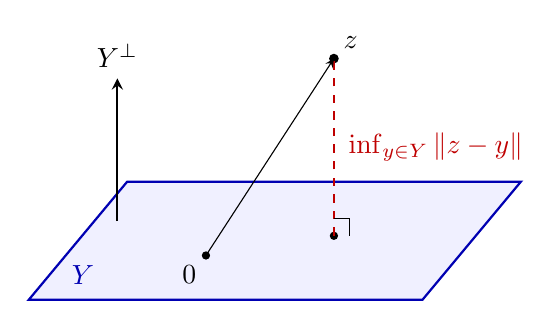
\begin{tikzpicture}[scale=1.25, >=stealth]
    \fill[blue!6] (-2.4,-0.7) -- (1.6,-0.7) -- (2.6,0.5) -- (-1.4,0.5) -- cycle;
    \draw[thick, blue!70!black] (-2.4,-0.7) -- (1.6,-0.7) -- (2.6,0.5) -- (-1.4,0.5) -- cycle;
    \node[blue!70!black] at (-1.85,-0.45) {$Y$};
    \fill (-0.6,-0.25) circle (1.2pt) node[below left] {$0$};
    \coordinate (P) at (0.7,-0.05);
    \coordinate (Z) at (0.7,1.75);
    \fill (Z) circle (1.4pt) node[above right] {$z$};
    \fill (P) circle (1.2pt);
    \draw[dashed, thick, red!75!black] (P) -- (Z);
    \node[red!75!black, anchor=west, align=left] at (0.75,0.85) {$\inf_{y \in Y} \|z - y\|$};
    \draw (P) ++(0,0.18) -- ++(0.16,0) -- ++(0,-0.18);
    \draw[->, thick] (-1.5,0.1) -- (-1.5,1.55) node[above] {$Y^\perp$};
    \draw[->] (-0.6,-0.25) -- (Z);
\end{tikzpicture}
